\subsubsection{Rancangan Detail Komponen Testing}
\label{subsubsection:detail-data-testing}

Komponen \textit{testing} bertanggung jawab untuk melakukan pengujian terhadap sistem yang telah dibangun. Pengujian ini dilakukan untuk memastikan bahwa sistem berfungsi sesuai dengan spesifikasi yang telah ditentukan. Komponen ini juga bertanggung jawab untuk menghasilkan data yang kemudian dimasukkan ke komponen \textit{reporting} untuk visualisasi dan analisis.

Ilustrasi struktur komponen \textit{testing} dapat dilihat pada gambar \ref{fig:testing-structure}.

% _TODO: Change image
\begin{figure}[ht]
    \centering
    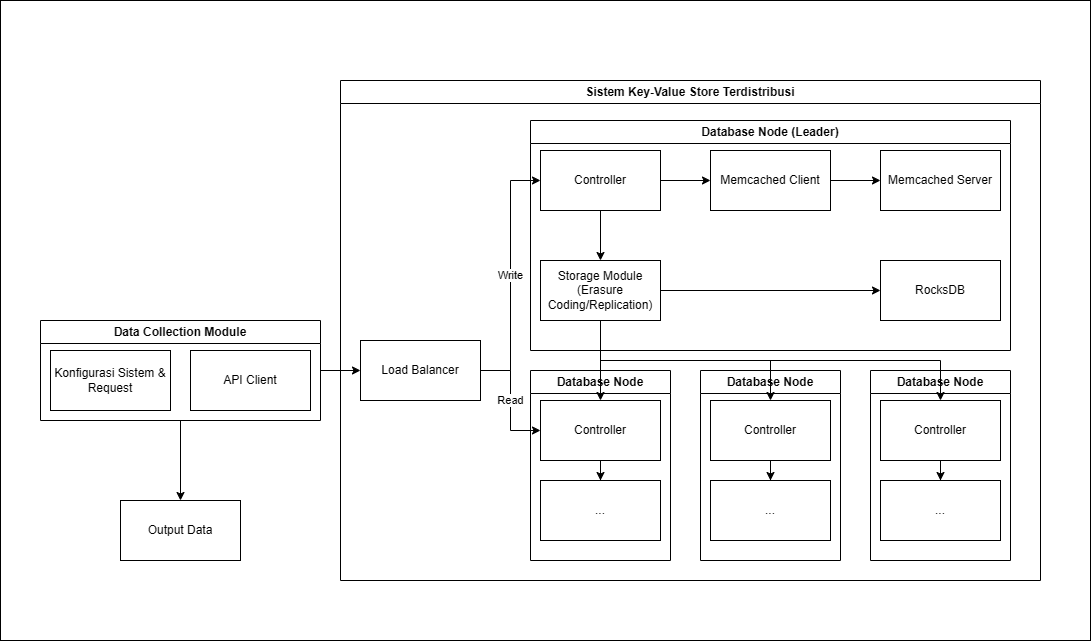
\includegraphics[width=0.95\textwidth]{resources/chapter-3/general-architecture.png}
    \caption{Struktur Komponen Testing}
    \label{fig:testing-structure}
\end{figure}